%----------------------------------------------------------------------------
\chapter{A JPorta (5-10 oldal)}\label{chapter:jporta}
%----------------------------------------------------------------------------

A BME Irányítástechnika és Informatika Tanszékén 2009 és 2015 között aktívan használták a CPorta névre keresztelt automatikus feladatkiértékelő rendszert, melyet a Közigazgatási Informatikai Központ (BME-IK) munkatársai fejlesztettek. Az idő folyamán a rendszert folyamatosan bővítették, azonban egy idő után ez egyre nehézkesebbé vált. Ennek oka a fejlesztőgárda cserélődése, a nem megfelelően átgondolt új funkciók implementálása, illetve az igények változása volt. Ezek miatt 2014-ben új portál fejlesztését kezdték meg a tanszéken \cite{KalmanMsc}.

 Így született meg a JPorta névre keresztelt oktatás támogató és automatikus feladatkiértékelő rendszer. A rendszer implementálása a Python programnyelv 3-as verziójával valósult meg, ezzel biztosítva a tartós támogatottságot. A webes felület generálásáért pedig a Django \cite{Django} keretrendszer 1.11.5-ös verzióját használja jelenleg, amely ezen felül felelős a belső adatmodellen végzett műveletek adatbázisműveletekre fordításáért és végrehajtásáért is. 

 \section{Alapvető felépítés}

    A JPorta keretein belül a Neptun rendszerhez hasonló tárgy-kurzus struktúra került implementálásra. Ezáltal létrehozhatóak tárgyak, majd ezeken belül további kurzusok a gyakorlatok és a laboratóriumi foglalkozások számára (ld. \ref{fig:jporta_course}. ábra). A tárgyakhoz és a kurzusokhoz külön-külön rendelhetünk oktatókat, hallgatókat viszont csak az utóbbihoz. Az kurzusokhoz rendelt oktatóknak van lehetősége az adott csoport hallgatóit értékelni, jelenléteiket adminisztrálni, beadásaikat megtekinteni és körlevelet írni a tagoknak. A tárgyhoz rendelt oktatónak ezen felül joga van minden tárgy szintű adminisztrációhoz is.

     \begin{figure}[h]
        \centering
        \resizebox{\textwidth}{!}{
            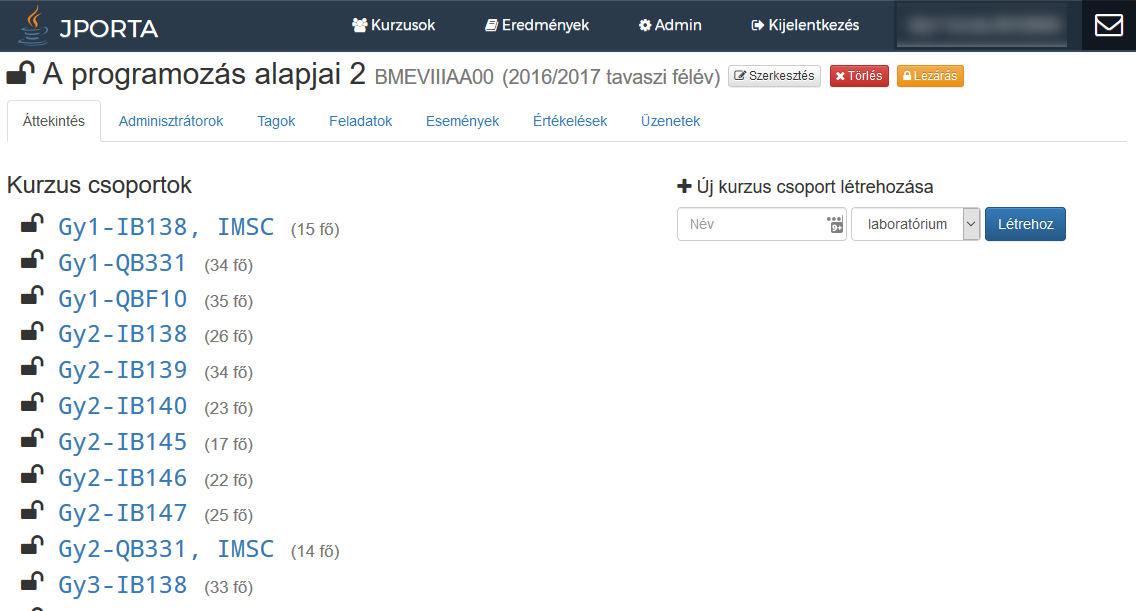
\includegraphics[]{jporta_course.png}
        }
        \caption{Tárgy adminisztrációs nézet a kurzusokkal}
        \label{fig:jporta_course}
    \end{figure}    

    A kurzusokhoz hozzárendelhetünk különböző számonkérések és jelenlétek eredményét (ld. \aref{fig:jporta_results}. ábra), ezekből készített dinamikusan számolódó mezőket, illetve automatikusan kiértékelődő feladatokat. Ezekről részletesebben \aref{chapter:assessments}. és \aref{chapter:exercise}. fejezetben lesz szó.

    \begin{figure}[h]
        \centering
        \resizebox{\textwidth}{!}{
            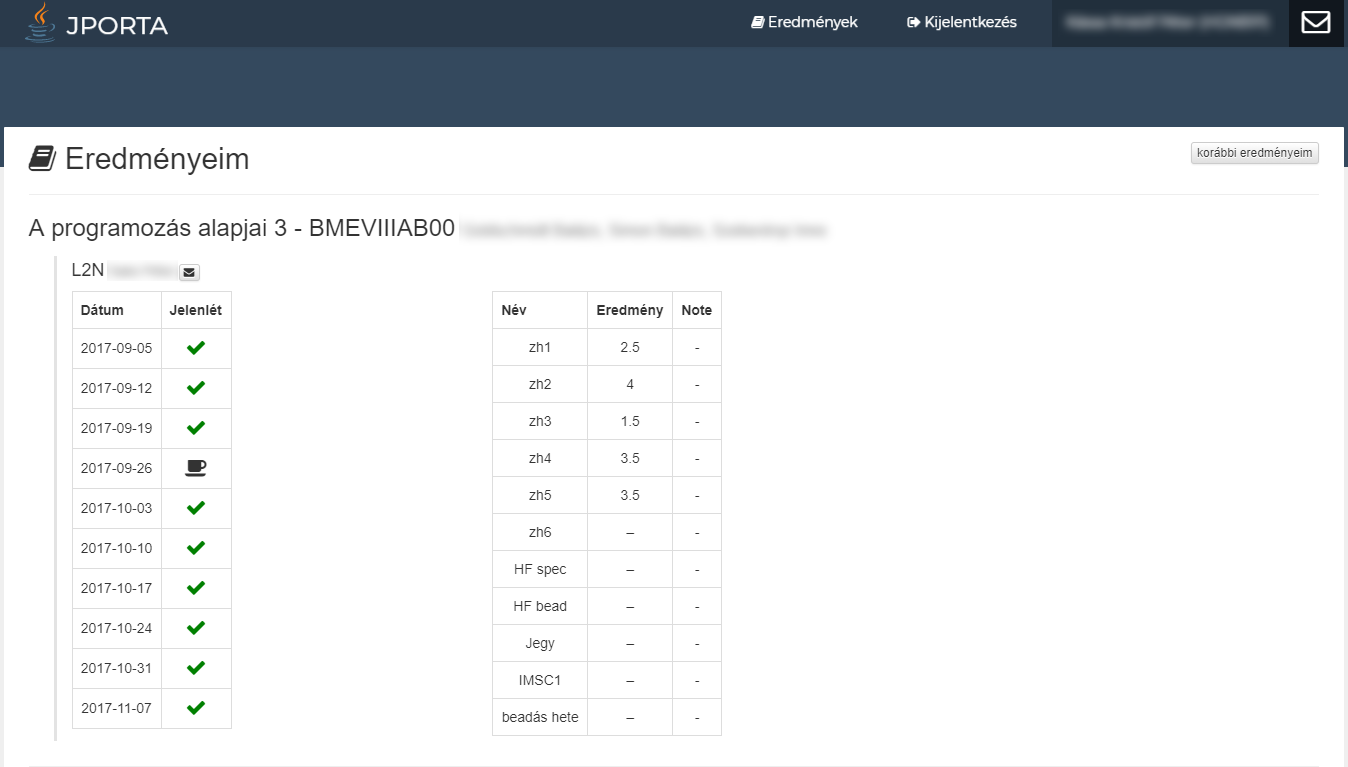
\includegraphics[]{jporta_results.png}
        }
        \caption{Eredmények egy hallgató szemszögéből}
        \label{fig:jporta_results}
    \end{figure} 

    A portálon jelenleg a be nem jelentkezett felhasználóknak nincs elérhető tartalom, így első lépés a kötelező authentikáció. Erre jelenleg két mód áll rendelkezésre:

    \begin{itemize}
        \item BME címtár azonosítás \cite{BMECimtar}: ez az elsődleges azonosítási forma, ugyanis a célközönséget képző hallgatók és oktatók mind rendelkeznek ilyen fiókkal. Ennek köszönhetően egyszerűen, külön regisztráció nélkül hiteles adatokhoz juthatunk.
        \item Hagyományos felhasználói név és jelszó pár: ez a hitelesítési mód ritkán, csak kivételes esetekben használt. Ilyen lehet a portál bemutatására szánt próba felhasználói fiók.
    \end{itemize}

    A bejelentkezett felhasználók szerepelhetnek egyes tárgyaknál oktatói, másoknál hallgatói szerepben. Erre sok esetben szükség is van, hiszen a laboratóriumi foglalkozásokat és gyakorlatokat gyakran felsőbb éves hallgatók tartják. Az oktatók jogairól és egyéb lehetőségeiról részletesebben \aref{section:teacher}. fejezetben lesz szó.
     
\section{A rendszer hallgatói oldalról}
    A portálra belépve a hallgatókat egy összefoglaló nézet fogadja (ld. \aref{fig:jporta_home}. ábra). Itt találnak egy összefoglalót az aktuális és a már lejárt határidejű online beadandó feladataikról. Egy feladatot kiválasztva pedig lehetőségük nyílik annak beadására (ha a határidő még nem járt le) és az előző beadások részleteinek megtekintésére (ha vannak). Ilyen feladat többféle lehet, gyakran használtak az alábbiak:

    \begin{itemize}
        \item Dokumentum feltöltése: tipikusan, házi feladatok specifikációihoz, dokumentációihoz tartozóan, pdf formában.
        \item Programkód feltöltése: külön állományokban, vagy zip fájlban, mely több forrásfájlt is tartalmazhat. Ezeket a rendszer lefordítja, lefuttattja és ellenőrzi a futást, ha az előbbiek sikeresek voltak.
    \end{itemize}

    Természetesen nem csak ilyen blokkok létrehozására van lehetősége az oktatóknak. Ezek testreszabhatóságaira \aref{chapter:exercise}. fejezetben fogok részletesen kitérni.
    
    \begin{figure}[h]
        \centering
        \resizebox{\textwidth}{!}{
            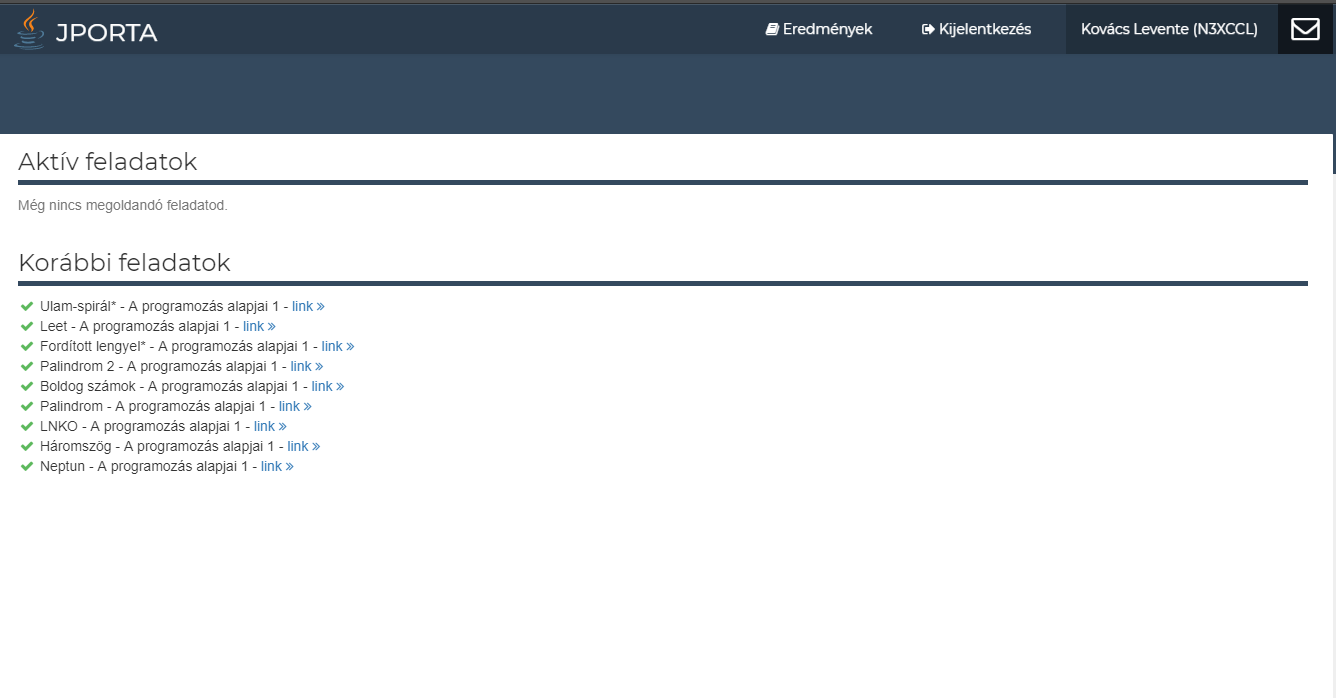
\includegraphics[]{jporta_home.png}
        }
        \caption{Belépő képernyő hallgatói szemszögből}
        \label{fig:jporta_home}
    \end{figure}

    Innen továbbnavigálva a hallgatók megtekinthetik részletesen az aktuális és korábbi félévekben regisztrált eredményeiket, jelenléteiket. A portál ezen felül egyszerűsíti a hallgatók és oktatók közötti kommunikációt üzenetküldési funkcióval, így nincs szükség a másik fél e-mail címének ismerésére. Minden így küldött üzenetről a címzett automatikus e-mail formájában is értesül, azonban a válasz csak a felületről lehetséges.
 
\section{A rendszer oktatói oldalról}\label{section:teacher}
    Az oktatóknak lehetősége van a tárgyukhoz vagy kurzusukhoz tartozó hallgatók értékelésére, feladatok kiírására és körüzenet küldésére. Az értékelésbe beletartozik a különböző zárthelyi dolgozatok eredményének és az órai jelenlétek vezetése, illetve az automatikusan kiértékelődő feladatok ellenőrzése, esetleges felülbírálása.

    A tárgy oktatói tudnak kurzusokat létrehozni, azokba hallgatókat felvenni. Emellett folyamatosan van lehetőségük új értékelések és automatikusan kiértékelődő feladatok hozzáadására. Ezek hozzáadása után a kurzusok oktatói fogják az eredményeket regisztrálni és a beadott feladatokat ellenőrizni, esetlegesen az automatikus értékelést felülbírálni.

\section{Modulok felépítése}